\documentclass[notes,11pt, aspectratio=169]{beamer}


% slide format copied from Paul Goldsmith-Pinkham

\usepackage{pgfpages}
% These slides also contain speaker notes. You can print just the slides,
% just the notes, or both, depending on the setting below. Comment out the want
% you want.
\setbeameroption{hide notes} % Only slide
%\setbeameroption{show only notes} % Only notes
%\setbeameroption{show notes on second screen=right} % Both

\usepackage{helvet}
\usepackage[default]{lato}
\usepackage{array}
\usepackage{tgbonum}

\usepackage{tikz}
\usepackage{verbatim}
\setbeamertemplate{note page}{\pagecolor{yellow!5}\insertnote}
\usetikzlibrary{positioning}
\usetikzlibrary{snakes}
\usetikzlibrary{calc}
\usetikzlibrary{arrows}
\usetikzlibrary{decorations.markings}
\usetikzlibrary{shapes.misc}
\usetikzlibrary{matrix,shapes,arrows,fit,tikzmark}
\usepackage{amsmath}
\usepackage{mathpazo}
\usepackage{hyperref}
\usepackage{lipsum}
\usepackage{multimedia}
\usepackage{graphicx}
\usepackage{multirow}
\usepackage{graphicx}
\usepackage{dcolumn}
\usepackage{bbm}
\usepackage{colortbl} % Add the colortbl package for coloring rows

\newcolumntype{d}[0]{D{.}{.}{5}}

\usepackage{changepage}
\usepackage{appendixnumberbeamer}

\usepackage{graphicx}
\usepackage[space]{grffile}
\usepackage{booktabs}

%AC citation
\usepackage{natbib}
\bibliographystyle{abbrvnat}
\setcitestyle{authordate,open={(},close={)}}


% These Andie Creels colors 
\definecolor{blue}{RGB}{76,173,205}
\definecolor{red}{RGB}{251,0,7}
\definecolor{yellow}{RGB}{238,158,9}
\definecolor{green}{RGB}{18,145,118}


%AC: Shifting title down 
% \makeatletter
% \setbeamertemplate{frametitle}{
%     \ifbeamercolorempty[bg]{frametitle}{}{\nointerlineskip}%
%     \@tempdima=\textwidth%
%     \advance\@tempdima by\beamer@leftmargin%
%     \advance\@tempdima by\beamer@rightmargin%
%     \vspace{1.5cm} %%%%%%%%%%%%% SHIFTING DOWN 
%     \begin{beamercolorbox}[sep=0.3cm,,wd=\the\@tempdima]{frametitle}
%         \usebeamerfont{frametitle}%
%         \vbox{}\vskip-1ex%
%         \if@tempswa\else\csname beamer@ftecenter\endcsname\fi%
%         \strut\insertframetitle\strut\par%
%         {%
%             \ifx\insertframesubtitle\@empty%
%             \else%
%             {\usebeamerfont{framesubtitle}\usebeamercolor[fg]{framesubtitle}\insertframesubtitle\strut\par}%
%             \fi
%         }%
%         \vskip-1ex%
%         \if@tempswa\else\vskip-.3cm\fi% set inside beamercolorbox... evil here...
%     \end{beamercolorbox}%
% }
% \makeatother



\hypersetup{
  colorlinks=false,
  linkbordercolor = {white},
  linkcolor = {blue}
}


%% PGP uses a beige off white for my background
\definecolor{MyBackground}{RGB}{255,253,218}

%% Uncomment this if you want to change the background color to something else (Andie uses white for background)
%\setbeamercolor{background canvas}{bg=MyBackground}

%% Change the bg color to adjust your transition slide background color!
\newenvironment{transitionframe}{
  \setbeamercolor{background canvas}{bg=yellow}
  \begin{frame}}{
    \end{frame}
}

\setbeamercolor{frametitle}{fg=black}
\setbeamercolor{title}{fg=black}
\setbeamertemplate{footline}[frame number]
\setbeamertemplate{navigation symbols}{} 
\setbeamertemplate{itemize items}{-}
\setbeamercolor{itemize item}{fg=black}
\setbeamercolor{itemize subitem}{fg=black}
\setbeamercolor{enumerate item}{fg=black}
\setbeamercolor{enumerate subitem}{fg=black}
\setbeamercolor{button}{bg=MyBackground,fg=black,}



% If you like road maps, rather than having clutter at the top, have a roadmap show up at the end of each section 
% (and after your introduction)
% Uncomment this is if you want the roadmap!
% \AtBeginSection[]
% {
%    \begin{frame}
%        \frametitle{Roadmap of Talk}
%        \tableofcontents[currentsection]
%    \end{frame}
% }
\setbeamercolor{section in toc}{fg=green}
\setbeamercolor{subsection in toc}{fg=blue}
\setbeamersize{text margin left=1em,text margin right=1em} 

\newenvironment{wideitemize}{\itemize\addtolength{\itemsep}{10pt}}{\enditemize}

\usepackage{environ}
\NewEnviron{videoframe}[1]{
  \begin{frame}
    \vspace{-8pt}
    \begin{columns}[onlytextwidth, T] % align columns
      \begin{column}{.70\textwidth}
        \begin{minipage}[t][\textheight][t]
          {\dimexpr\textwidth}
          \vspace{8pt}
          \hspace{4pt} {\Large \sc \textcolor{blue}{#1}}
          \vspace{8pt}
          
          \BODY
        \end{minipage}
      \end{column}%
      \hfill%
      \begin{column}{.38\textwidth}
        \colorbox{green!20}{\begin{minipage}[t][1.2\textheight][t]
            {\dimexpr\textwidth}
            Face goes here
          \end{minipage}}
      \end{column}%
    \end{columns}
  \end{frame}
}

% AC: Background for title slide
% \pgfdeclareimage[width=\paperwidth]{bridger}{bridger-dallas.jpg}
% \usebackgroundtemplate{\tikz\node[opacity=0.3, ,inner sep=0] {\pgfuseimage{bridger}};}


\title[]{\textcolor{black}{\textbf{National Aggregate Value of Local Outdoor Recreation}}
\subtitle{Achieving repeatable statistical products using ATUS}}
\author[]{Andie Creel}
\institute[]{\small{Camp Resources}}
\date{August 7, 2023}

% --------------------
% FUNCTIONS 
% --------------------

% Define a new command to highlight the second row with grey
\newcommand{\highlightrow}[1]{\only<#1>{\rowcolor{gray!20}}}


\begin{document}

%%% TIKZ STUFF
\tikzset{   
        every picture/.style={remember picture,baseline},
        every node/.style={anchor=base,align=center,outer sep=1.5pt},
        every path/.style={thick},
        }
\newcommand\marktopleft[1]{%
    \tikz[overlay,remember picture] 
        \node (marker-#1-a) at (-.3em,.3em) {};%
}
\newcommand\markbottomright[2]{%
    \tikz[overlay,remember picture] 
        \node (marker-#1-b) at (0em,0em) {};%
}
\tikzstyle{every picture}+=[remember picture] 
\tikzstyle{mybox} =[draw=black, very thick, rectangle, inner sep=10pt, inner ysep=20pt]
\tikzstyle{fancytitle} =[draw=black,fill=red, text=white]
%%%% END TIKZ STUFF

% Title Slide
\begin{frame}
\maketitle
\end{frame}

% ------------------------------ 
% MOTIVATION
% ------------------------------ 
% image
% \pgfdeclareimage[width=\paperwidth]{slide1}{park-people-nyc.jpg}
% \usebackgroundtemplate{\tikz\node[opacity=0.2, ,inner sep=0] {\pgfuseimage{slide1}};}

%slide
\begin{frame}{Motivation}

\begin{columns}[T] % align columns
\begin{column}{.9\textwidth}
  \begin{wideitemize}
  \item Sustainable development: non-declining welfare for future generations 
  \item Wealth is proportional to welfare \citep{arrow_evaluating_2003}
  \item Biden Administration wants to account for natural capital (wealth)
  \item  Outdoor recreation is a major service provided by natural capital 
  \item Contribution: 
    \begin{enumerate}
        \item An easily repeatable statistical product measuring value of local outdoor recreation
        \item Inform Census Bureau/BLS on additional questions that could easily be included so ATUS can inform national accounts of environmental stats 
    \end{enumerate}

  \end{wideitemize}
\end{column}%
\hfill%
\begin{column}{.38\textwidth}
  \makebox[\linewidth][c]{
    \resizebox{\linewidth}{!}{
%      \includegraphics{how-to-draw-an-owl.pdf}
    }
  }
\end{column}%
\end{columns}
\end{frame}

% ------------------------------ 
% LOCAL OUTDOOR RECREATION
% ------------------------------ 
% image
% \pgfdeclareimage[width=\paperwidth]{slide1}{park-people-nyc.jpg}
% \usebackgroundtemplate{\tikz\node[opacity=0.2, ,inner sep=0] {\pgfuseimage{slide1}};}

%slide
\begin{frame}{Local Recreation}

\begin{columns}[T] % align columns
\begin{column}{.9\textwidth}
  \begin{wideitemize}
  \item There is no comprehensive evaluation of local parks' contribution to the nation's welfare 
      \begin{itemize}
          \item Hindrance has been data, but ATUS data can be used for this \citep{berry_allocation_2018} 
          \item Many excellent local or regional studies, but none national in scope 
      \end{itemize}
  \item BEA/DOI analysis of the recreation industry's contribution to the economy doesn't include activities within 50 miles of home 
  % \begin{itemize}
  %     \item Expenditure account, which is included in the GDP 
  %     \item Our scope would be outside of GDP, but should be included in a wealth account (similar to household-produced services)
  % \end{itemize}

  \item Average travel time to recreate outdoors is 12 minutes (ATUS Data) 
  \item \textbf{Goal: Estimate the welfare contribution of local outdoor recreation using the ATUS data and easily repeated methods. }

  \end{wideitemize}
\end{column}%
\hfill%
\begin{column}{.38\textwidth}
  \makebox[\linewidth][c]{
    \resizebox{\linewidth}{!}{
%      \includegraphics{how-to-draw-an-owl.pdf}
    }
  }
\end{column}%
\end{columns}
\end{frame}

% ------------------------------ 
% DATA
% ------------------------------ 
% image
% \pgfdeclareimage[width=\paperwidth]{slide1}{park-people-nyc.jpg}
% \usebackgroundtemplate{\tikz\node[opacity=0.2, ,inner sep=0] {\pgfuseimage{slide1}};}

%slide
\begin{frame}{Data}

\begin{columns}[T] % align columns
\begin{column}{.4\textwidth}
  \begin{wideitemize}
  \item American Time Use Survey: 
    \begin{itemize}
        \item Representative spatial coverage
        \item Conducted since 2003
        \item 48 outdoor leisure activities
        % (9 pages of activity codes)
        \item Travel time
    \end{itemize}  
  \item Essentially long by minute 


  \end{wideitemize}
\end{column}%
\hfill%
\begin{column}{.58\textwidth}
  \makebox[\linewidth][c]{
    \resizebox{\linewidth}{!}{
     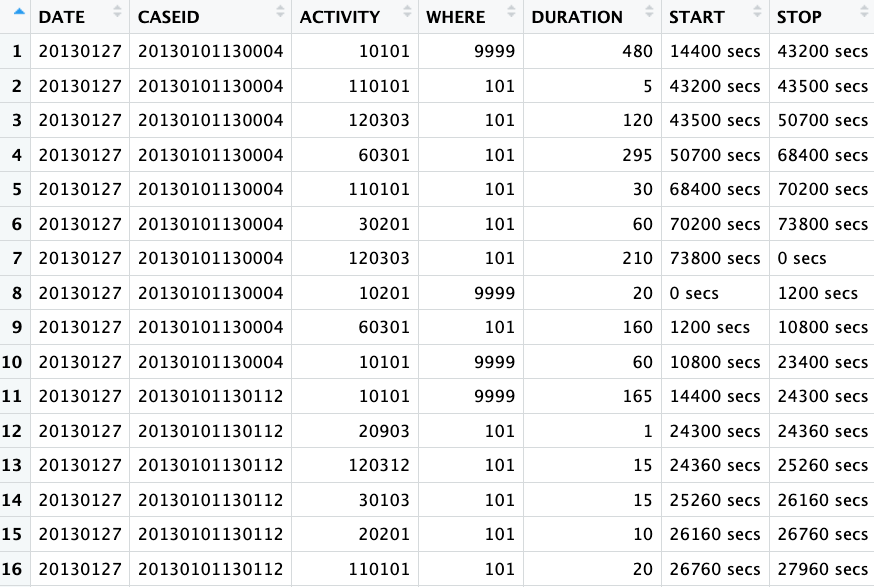
\includegraphics{data.png}
    }
  }
\end{column}%
\end{columns}
\end{frame}



% ------------------------------ 
% SUMMARY STATS 
% ------------------------------ 
% image
% \pgfdeclareimage[width=\paperwidth]{slide1}{park-people-nyc.jpg}
% \usebackgroundtemplate{\tikz\node[opacity=0.2, ,inner sep=0] {\pgfuseimage{slide1}};}

%slide
\begin{frame}{Summary Statistics}

    \begin{table}
    \caption{Percent of Americans Participating by Season}
    \centering
    \begin{tabular}[t]{lllll}
    \toprule
    activity & spring & summer & fall & winter\\
    \midrule
    indoor home & 97 & 97 & 98 & 98\\
    indoor away & 52 & 51 & 51 & 50\\
    \highlightrow{2} % Add this command before the row you want to highlight
    outdoor away & 9 & 10 & 7 & 7\\
    outdoor home & 6 & 7 & 4 & 4\\
    n & 3,942,400 & 3,906,000 & 3,842,160 & 3,979,520\\
    \bottomrule
    \end{tabular}
    \end{table}
\end{frame}

% ------------------------------ 
% SUMMARY STATS 
% ------------------------------ 
% image
% \pgfdeclareimage[width=\paperwidth]{slide1}{park-people-nyc.jpg}
% \usebackgroundtemplate{\tikz\node[opacity=0.2, ,inner sep=0] {\pgfuseimage{slide1}};}

%slide
\begin{frame}{Summary Statistics}
\begin{columns}[T] % align columns
\begin{column}{\textwidth}
    \begin{figure}
    \centering
    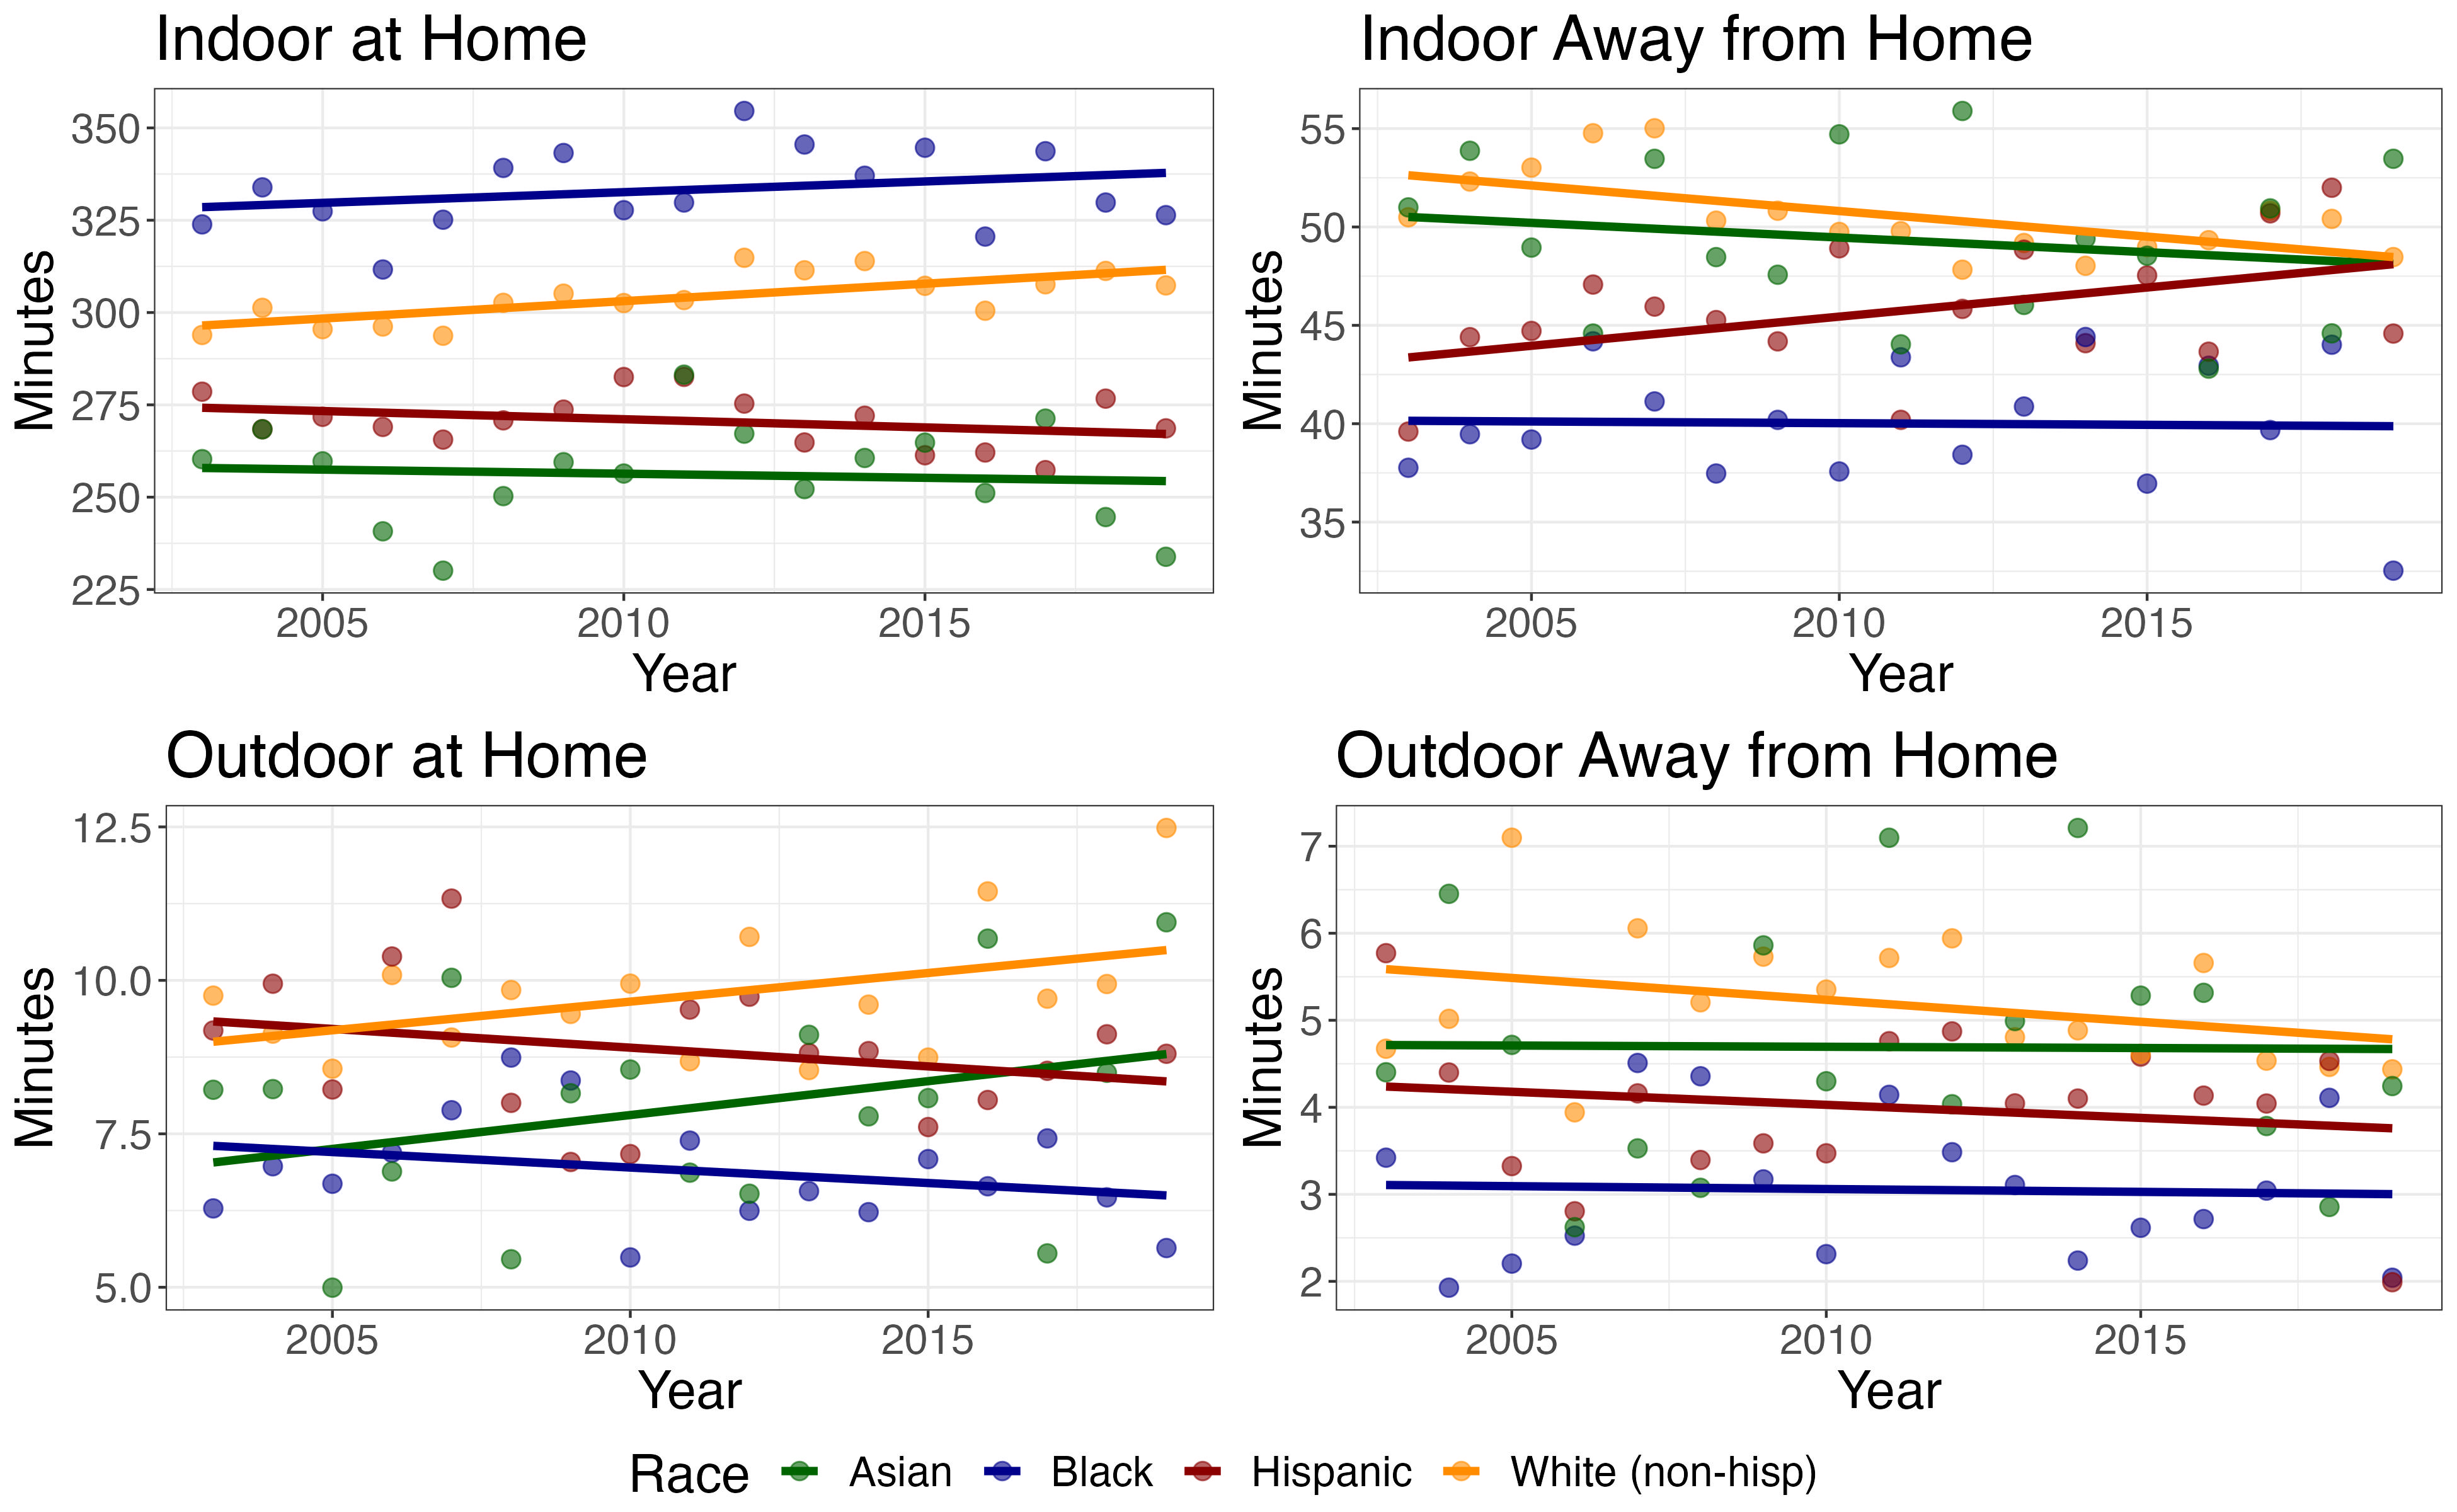
\includegraphics[height=0.85\textheight]{minutes_per_day.jpeg}
    % \caption{Caption for the image}
    \end{figure}
\end{column}%
\hfill%
\begin{column}{0.58\textwidth}
  \makebox[\linewidth][c]{
    \resizebox{\linewidth}{!}{
     % 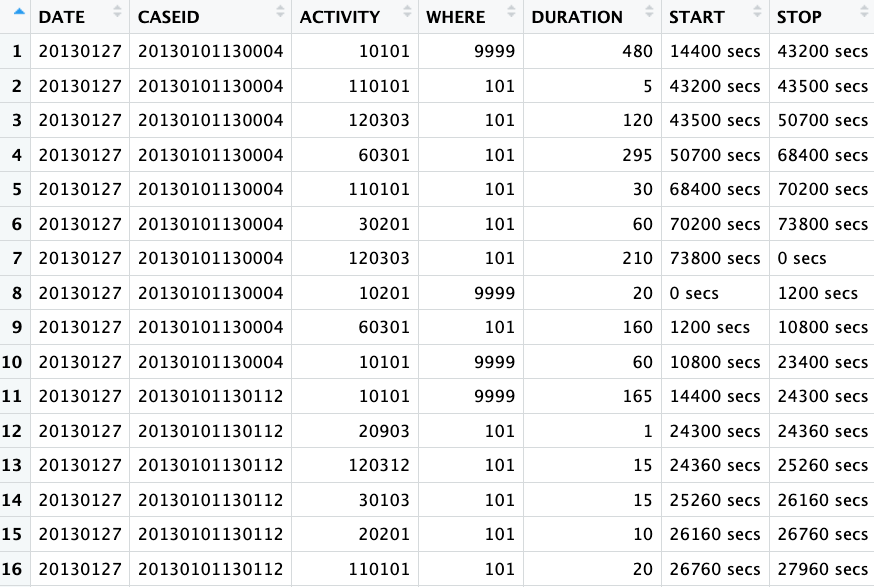
\includegraphics{data.png}
    }
  }
\end{column}%
\end{columns}
\end{frame}


% ------------------------------ 
% Random Utility Model 
% ------------------------------ 
% image
% \pgfdeclareimage[width=\paperwidth]{slide1}{park-people-nyc.jpg}
% \usebackgroundtemplate{\tikz\node[opacity=0.2, ,inner sep=0] {\pgfuseimage{slide1}};}

%slide
\begin{frame}{Random Utility Model}

\begin{columns}[T] % align columns
\begin{column}{.9\textwidth}

  \begin{align}
    V_{ic} = \alpha_c + \beta x_{ic} + \epsilon_{ic}
  \end{align}
  
\begin{itemize}
    \item Indirect utility: $V$
    \item Choice specific constant: $\alpha$
    \item Travel time: $x$
    \item General coefficient for travel time: $\beta$
    \item Choice set of leisure activities: indoor at home, indoor away from home, outdoor at home, outdoor away from home
    \item Less than 1\% of respondents do not participate in at least one of these activities per day 
\end{itemize}





\end{column}%
\hfill%
\begin{column}{.38\textwidth}
  \makebox[\linewidth][c]{
    \resizebox{\linewidth}{!}{
%      \includegraphics{how-to-draw-an-owl.pdf}
    }
  }
\end{column}%
\end{columns}
\end{frame}

% ------------------------------ 
% WELFARE RESULT 
% ------------------------------ 
% image
% \pgfdeclareimage[width=\paperwidth]{slide1}{park-people-nyc.jpg}
% \usebackgroundtemplate{\tikz\node[opacity=0.2, ,inner sep=0] {\pgfuseimage{slide1}};}

%slide
\begin{frame}{Welfare Analysis }

\begin{columns}[T] % align columns
\begin{column}{.9\textwidth}
  \begin{wideitemize}
  \item What's the right counterfactual to use to calculate welfare? If all local parks were eliminated? 
  \item Send price to infinity? 
  \item introduce reiman sum idea?
  \item I want feedback here on tracing demand curve
  

  \end{wideitemize}
\end{column}%
\hfill%
\begin{column}{.38\textwidth}
  \makebox[\linewidth][c]{
    \resizebox{\linewidth}{!}{
%      \includegraphics{how-to-draw-an-owl.pdf}
    }
  }
\end{column}%
\end{columns}
\end{frame}

% ------------------------------ 
% EXTENSIONS
% ------------------------------ 
% image
% \pgfdeclareimage[width=\paperwidth]{slide1}{park-people-nyc.jpg}
% \usebackgroundtemplate{\tikz\node[opacity=0.2, ,inner sep=0] {\pgfuseimage{slide1}};}

%slide
\begin{frame}{Extensions}

\begin{columns}[T] % align columns
\begin{column}{.9\textwidth}
  \begin{wideitemize}
  \item Temperature analysis 
  \item Racial differences 
  \item cell phone data (stake flag) 
  

  \end{wideitemize}
\end{column}%
\hfill%
\begin{column}{.38\textwidth}
  \makebox[\linewidth][c]{
    \resizebox{\linewidth}{!}{
%      \includegraphics{how-to-draw-an-owl.pdf}
    }
  }
\end{column}%
\end{columns}
\end{frame}

% ------------------------------ 
% THANK YOU 
% ------------------------------ 
% image
% \pgfdeclareimage[width=\paperwidth]{slide1}{park-people-nyc.jpg}
% \usebackgroundtemplate{\tikz\node[opacity=0.2, ,inner sep=0] {\pgfuseimage{slide1}};}

%slide
\begin{frame}{Thank you }

\begin{columns}[T] % align columns
\begin{column}{.9\textwidth}
\begin{itemize}
    \item I would love your feedback and thoughts!  
    \item andie.creel@yale.edu
\end{itemize}
 
 
\end{column}%
\hfill%
\begin{column}{.38\textwidth}
  \makebox[\linewidth][c]{
    \resizebox{\linewidth}{!}{
%      \includegraphics{how-to-draw-an-owl.pdf}
    }
  }
\end{column}%
\end{columns}
\end{frame}


% ------------------------------ 
% BIBLIOGRAPHY 
% ------------------------------ 
\usebackgroundtemplate{}
\begin{frame}{Bibliography}
    \fontsize{7pt}{7pt}\selectfont
  \bibliography{bibliography_CR}
\end{frame}


\end{document}